%%%%%%%%%%%%%%%%%%%%%%%%%%%%%%%%%%%%%%%%%
% Beamer Presentation
% LaTeX Template
% Version 1.0 (10/11/12)
%
% This template has been downloaded from:
% http://www.LaTeXTemplates.com
%
% License:
% CC BY-NC-SA 3.0 (http://creativecommons.org/licenses/by-nc-sa/3.0/)
%
%%%%%%%%%%%%%%%%%%%%%%%%%%%%%%%%%%%%%%%%%

%----------------------------------------------------------------------------------------
%	PACKAGES AND THEMES
%----------------------------------------------------------------------------------------


%http://www.iep.utm.edu/mathplat/

\documentclass{beamer}

\mode<presentation> {

% The Beamer class comes with a number of default slide themes
% which change the colors and layouts of slides. Below this is a list
% of all the themes, uncomment each in turn to see what they look like.

%\usetheme{default}
%\usetheme{AnnArbor}
%\usetheme{Antibes}
%\usetheme{Bergen}
%\usetheme{Berkeley}
%\usetheme{Berlin}
%\usetheme{Boadilla}
%\usetheme{CambridgeUS}
%\usetheme{Copenhagen}
%\usetheme{Darmstadt}
%\usetheme{Dresden}
%\usetheme{Frankfurt}
%\usetheme{Goettingen}
%\usetheme{Hannover}
%\usetheme{Ilmenau}
%\usetheme{JuanLesPins}
%\usetheme{Luebeck}
\usetheme{Madrid}
%\usetheme{Malmoe}
%\usetheme{Marburg}
%\usetheme{Montpellier}
%\usetheme{PaloAlto}
%\usetheme{Pittsburgh}
%\usetheme{Rochester}
%\usetheme{Singapore}
%\usetheme{Szeged}
%\usetheme{Warsaw}

% As well as themes, the Beamer class has a number of color themes
% for any slide theme. Uncomment each of these in turn to see how it
% changes the colors of your current slide theme.

%\usecolortheme{albatross}
%\usecolortheme{beaver}
%\usecolortheme{beetle}
%\usecolortheme{crane}
%\usecolortheme{dolphin}
%\usecolortheme{dove}
%\usecolortheme{fly}
%\usecolortheme{lily}
%\usecolortheme{orchid}
%\usecolortheme{rose}
%\usecolortheme{seagull}
%\usecolortheme{seahorse}
%\usecolortheme{whale}
%\usecolortheme{wolverine}

%\setbeamertemplate{footline} % To remove the footer line in all slides uncomment this line
%\setbeamertemplate{footline}[page number] % To replace the footer line in all slides with a simple slide count uncomment this line

\setbeamertemplate{navigation symbols}{} % To remove the navigation symbols from the bottom of all slides uncomment this line
}

\usepackage{graphicx} % Allows including images
\usepackage{booktabs} % Allows the use of \toprule, \midrule and \bottomrule in tables
\usepackage{tipa}
\usepackage{amsmath}
\usepackage{physics}
\usepackage{siunitx}

\usepackage{multicol}
\usepackage{fancyvrb}
\fvset{fontsize=\normalsize}
\RecustomVerbatimEnvironment{verbatim}{Verbatim}{}
%----------------------------------------------------------------------------------------
%	TITLE PAGE
%----------------------------------------------------------------------------------------

\title[Quantenrechnung]{\textsc{Einführung in die Quantenrechnung} \\ Bits und Qubits} % The short title appears at the bottom of every slide, the full title is only on the title page

\author[bbphsgg@ma.eu]{Brian Benjamin Pomerantz und Henry Sebastian Graßhorn Gebhardt} % Your name
\institute[] % Your institution as it will appear on the bottom of every slide, may be shorthand to save space
{
P\&GG Monotechnische Anstalt\\ % Your institution for the title page
%\medskip
%\textit{bpomerantz@maizeanalytics.com} % Your email address
}
\date{2021 M\"arz 20 und 2021 April} % Date, can be changed to a custom date

\AtBeginSection[] {
\begin{frame}
\frametitle{Outline}
\tableofcontents[currentsection]
\end{frame}
}

\AtBeginSubsection[] {
\begin{frame}
\frametitle{Outline}
\tableofcontents[currentsection,currentsubsection]
\end{frame}
}

\begin{document}

\begin{frame}
\titlepage % Print the title page as the first slide
\end{frame}

\begin{frame}
\frametitle{Outline}
\tableofcontents
\end{frame}


\section{Einfache Computadoras}
\subsection{Mathematik}

\begin{frame}
\frametitle{Bin\"are Zahlen}
In decimal notation,
\begin{equation*}
1572_{10} = 1\times10^3 + \pause 5\times10^2 + \pause 7\times10^1 + \pause 2\times10^0
\end{equation*}
\pause
From binary to decimal,
\begin{align*}
1001101_2 &= 1\times2^6 + 1\times2^3 + 1\times2^2 + 1\times2^0 \\
&= 64 + 8 + 4 + 1 \\
&= 77_{10}
\end{align*}
\pause
Going from decimal to binary notation,
\begin{align*}
27_{10} &= 16 + 8 + 2 + 1 \\
&= 1\times2^4 + 1\times2^3 + 0\times2^2 + 1\times2^1 + 1\times2^0 \\
&= 11011_2
\end{align*}
\end{frame}

\begin{frame}
\frametitle{Powers von zwei}
\begin{align*}
	2^0 &= 1                 &= 000000001_2    \\
	2^1 &= \uncover<2->{ 2   &= 000000010_2   \\}
	2^2 &= \uncover<3->{ 4   &= 000000100_2  \\}
	2^3 &= \uncover<4->{ 8   &= 000001000_2 \\}
	2^4 &= \uncover<5->{ 16  &= 000010000_2 \\}
	2^5 &= \uncover<6->{ 32  &= 000100000_2 \\}
	2^6 &= \uncover<7->{ 64  &= 001000000_2 \\}
	2^7 &= \uncover<8->{ 128 &= 010000000_2 \\}
	2^8 &= \uncover<9->{ 256 &= 100000000_2}
\end{align*}
\end{frame}

\subsection{Architektur}

\begin{frame}
\frametitle{Logic Gates}
\begin{figure}
\centering
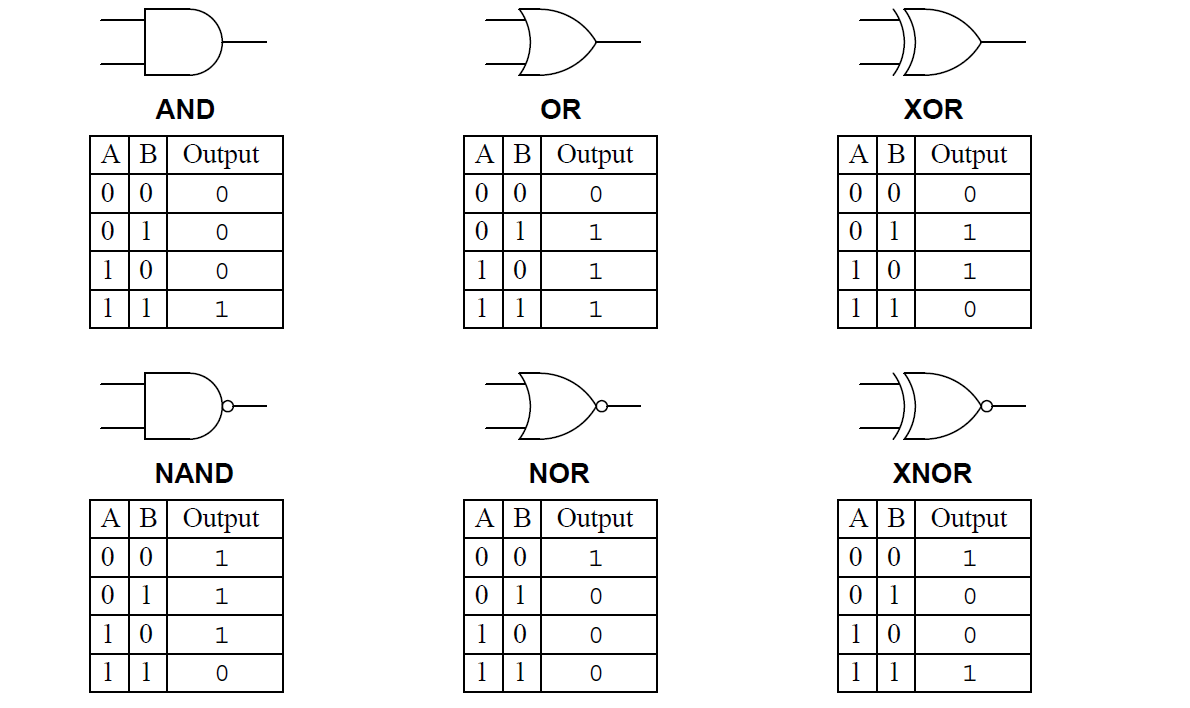
\includegraphics[width=\textwidth]{logic_gates.png}
\label{Logic Gates}
\end{figure}
\end{frame}

\begin{frame}
\frametitle{Adder}
\begin{figure}
\centering
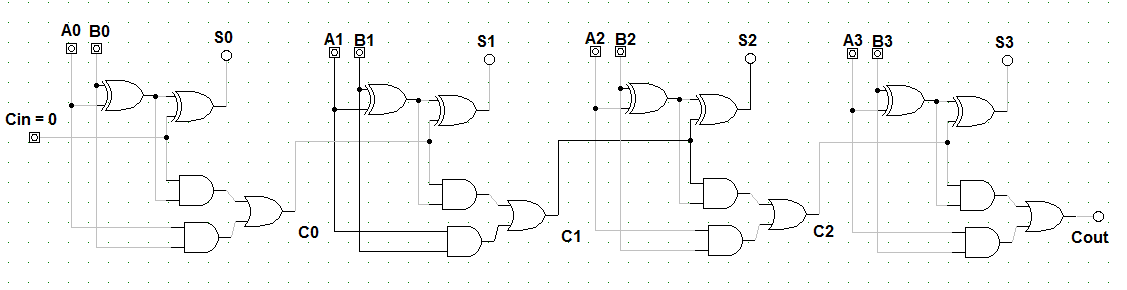
\includegraphics[width=\textwidth]{4bit_adder_3.png}
\label{Adder}
\end{figure}
\end{frame}

\begin{frame}
\frametitle{Computer Architektur}
\begin{figure}
\centering
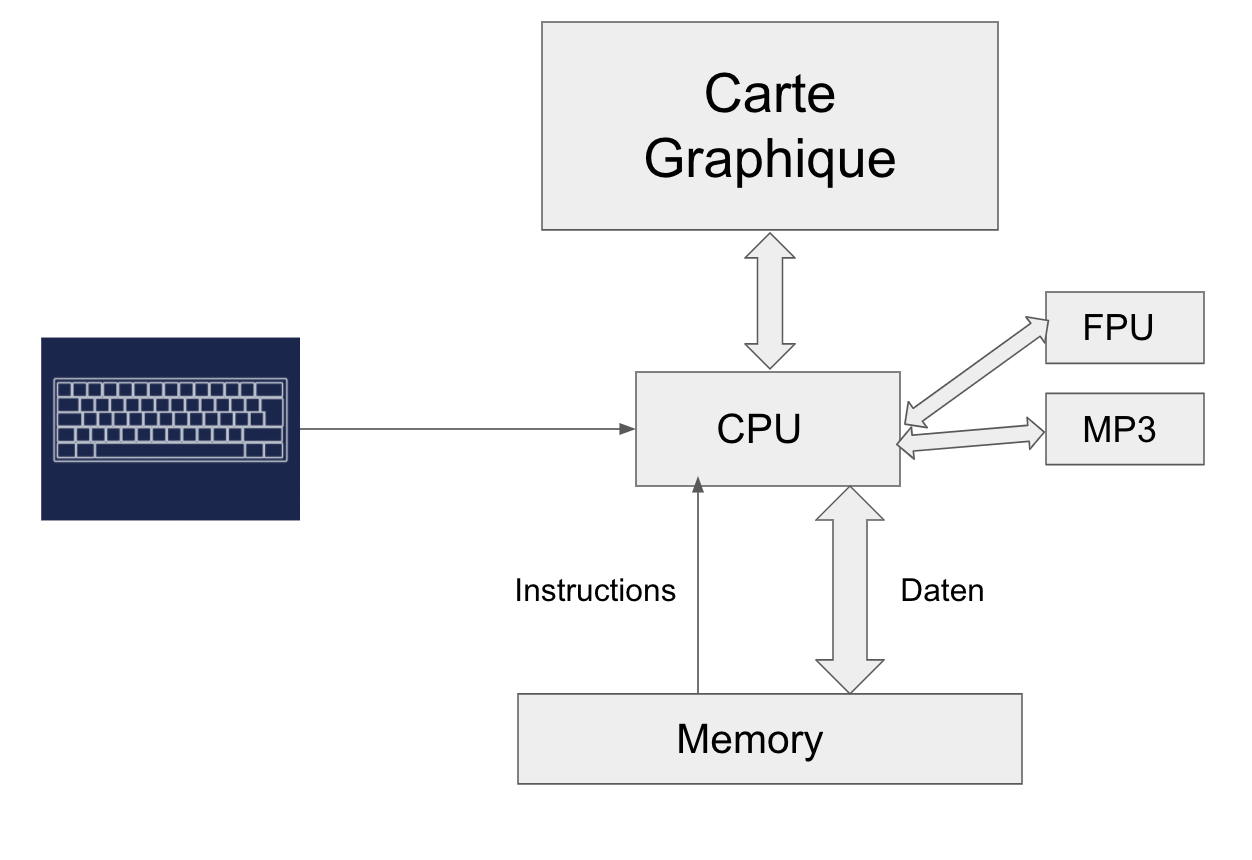
\includegraphics[width=\textwidth]{cpu.png}
\label{cpu}
\end{figure}
\end{frame}

\begin{frame}
\frametitle{Computer Architektur}
\begin{figure}
\centering
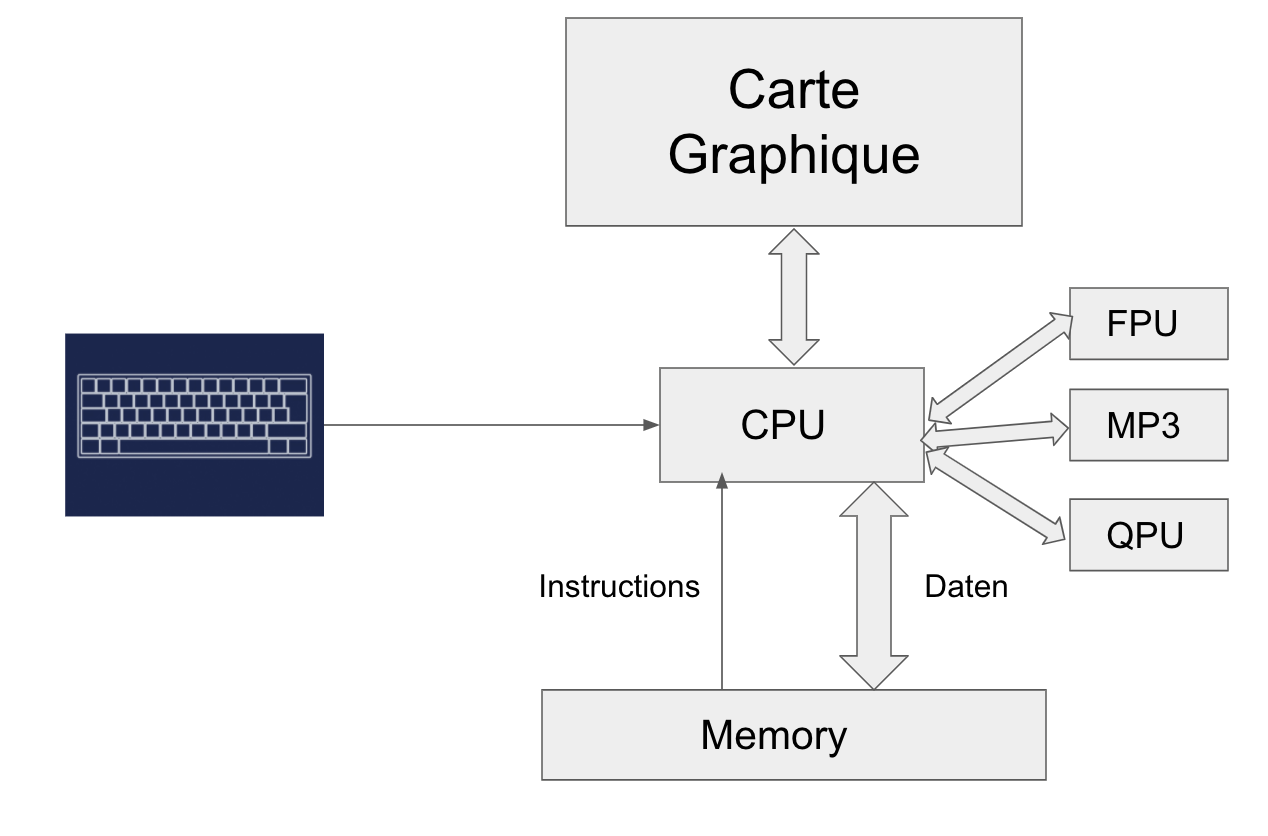
\includegraphics[width=\textwidth]{qpu.png}
\label{qpu}
\end{figure}
\end{frame}

\section{Computadora Cu\'antica: Eine schwarze Kunst}

\subsection{Quantenzust\"ande}

\begin{frame}
\frametitle{A QPU operates on Qubits instead of Bits}
\begin{itemize}
	\item QPU: Quantum Processing Unit
	\item Bits: 0, 1
	\item Qubits: $\ket{0}$, $\ket{1}$, and superpositions thereof
\end{itemize}
\end{frame}

\begin{frame}
\frametitle{Light is a wave}
\begin{figure}
\centering
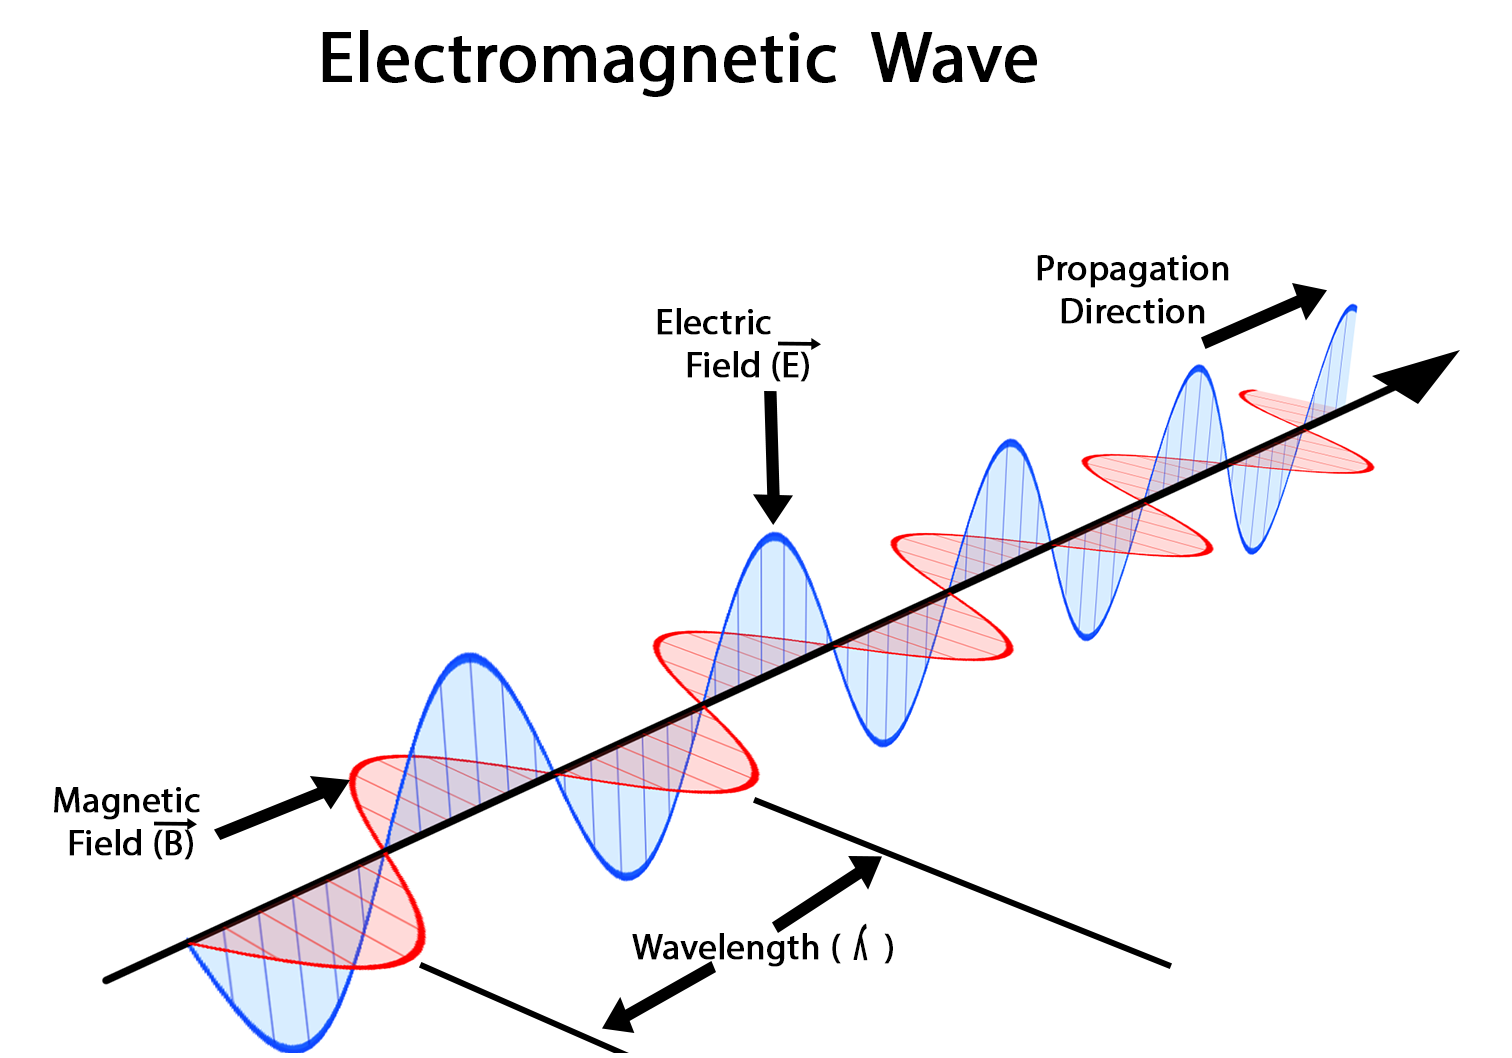
\includegraphics[width=\textheight,trim={0 0 0 190},clip]{light.png}
\label{polar1}
\end{figure}
\end{frame}

\begin{frame}
\frametitle{Polarization Experiment}
\begin{figure}
\centering
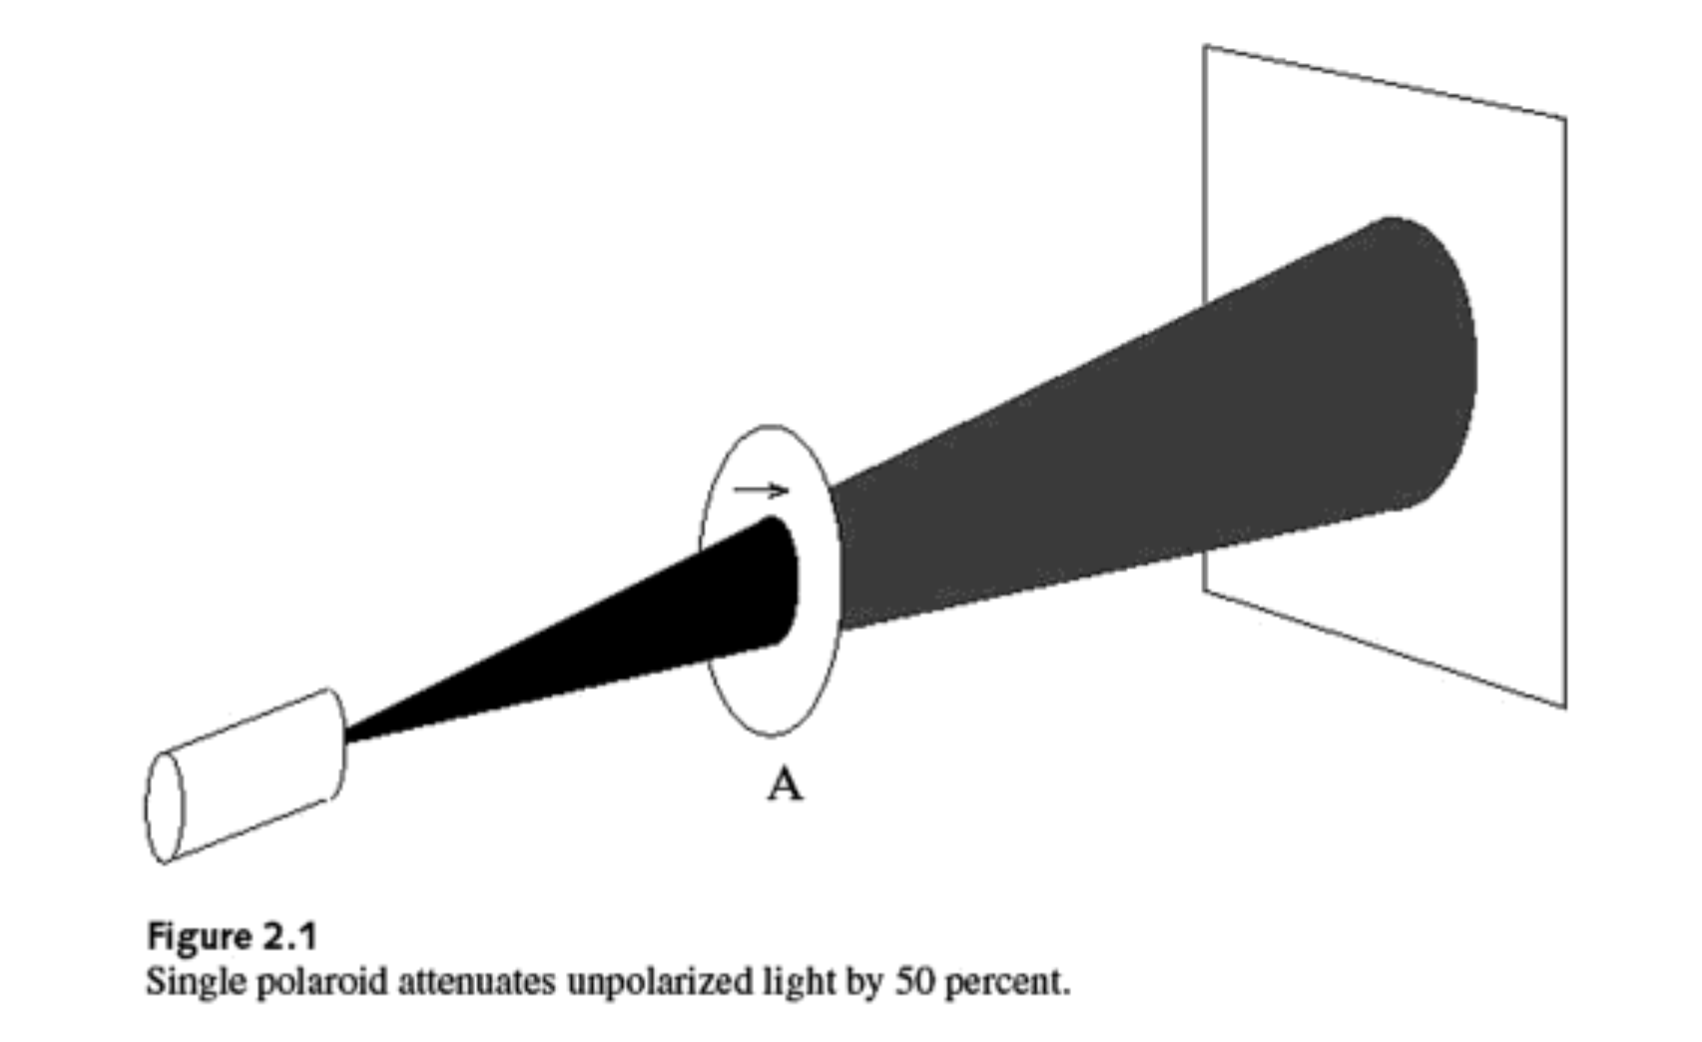
\includegraphics[width=\textwidth]{polar1.png}
\label{polar1}
\end{figure}
\end{frame}

\begin{frame}
\frametitle{Polarization Experiment}
\begin{figure}
\centering
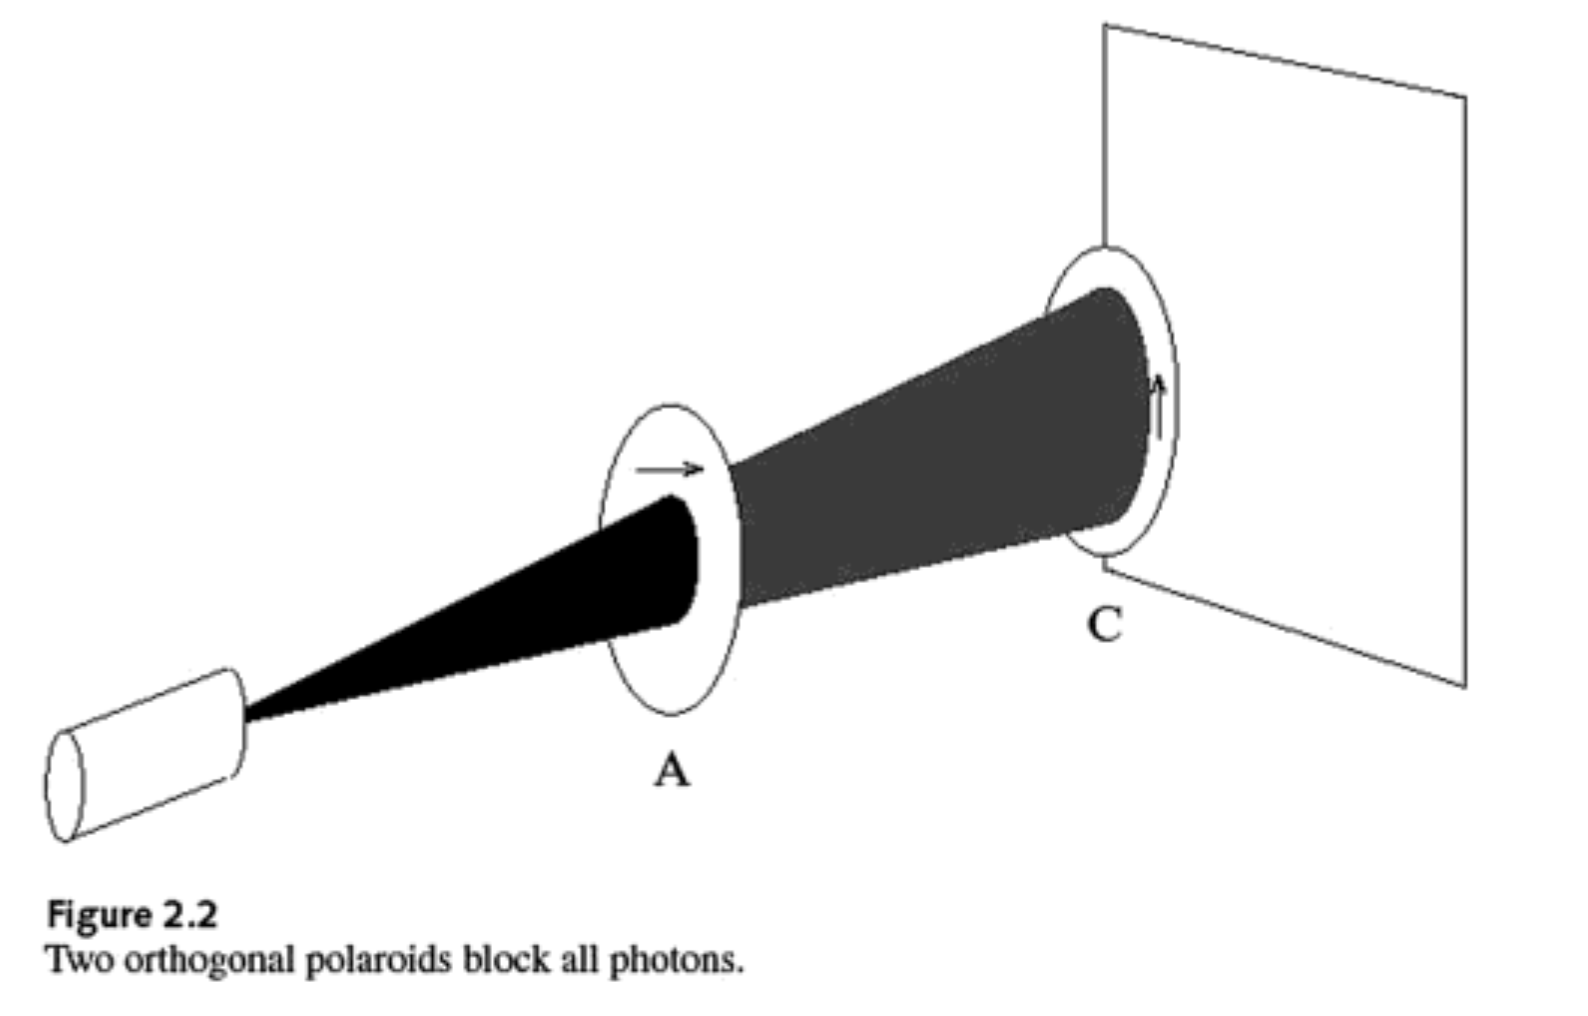
\includegraphics[width=\textwidth]{polar2.png}
\label{polar2}
\end{figure}
\end{frame}

\begin{frame}
\frametitle{Polarization Experiment}
\begin{figure}
\centering
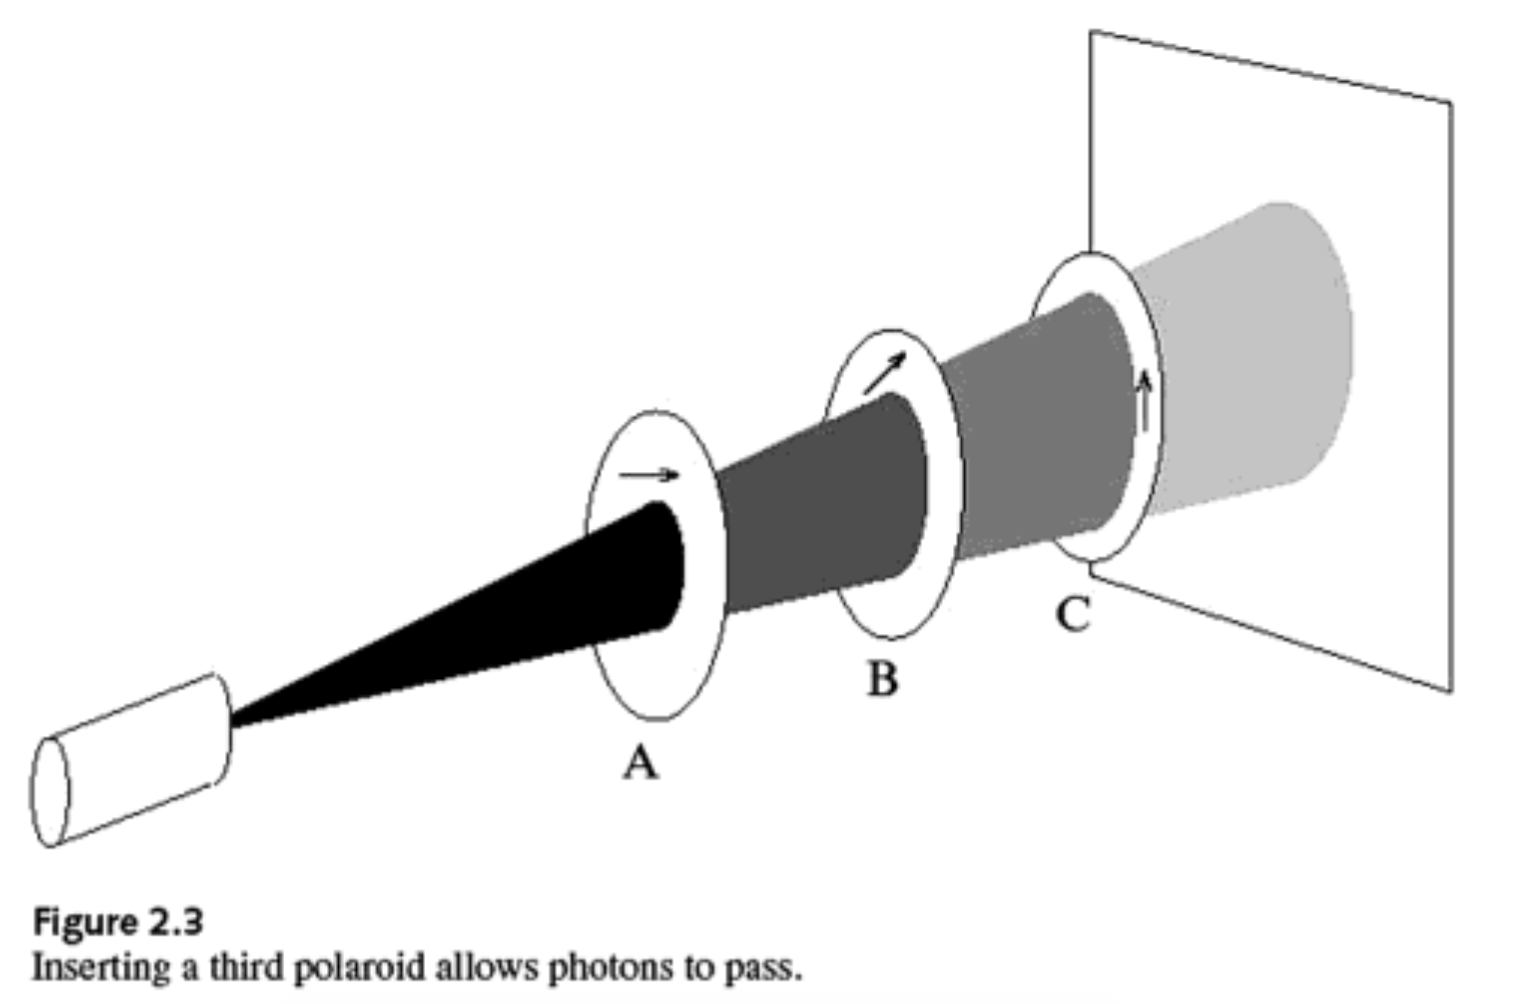
\includegraphics[width=\textwidth]{polar3.png}
\label{polar3}
\end{figure}
\end{frame}

\begin{frame}
\frametitle{Vektoren}
Alle Polarisationsrichtungen können durch zwei Vektoren dargestellt werden:
\begin{align*}
	\ket{\psi} &= a\ket{\to} + b\ket{\uparrow}
\end{align*}
Die Notation wird Bra-ket Notation genannt.

Beispiele:
\begin{align*}
	\ket{\SI{45}{\degree}} &= \frac{1}{\sqrt2}\ket{\to} + \frac{1}{\sqrt2}\ket{\uparrow}
	\\
	\ket{\SI{135}{\degree}} &= -\frac{1}{\sqrt2}\ket{\to} + \frac{1}{\sqrt2}\ket{\uparrow}
	\\
	\ket{\SI{30}{\degree}} &= \frac{1}{2}\ket{\to} + \frac{\sqrt3}{2}\ket{\uparrow}
	\\
	\ket{\theta} &= \sin\theta\ket{\to} + \cos\theta\ket{\uparrow}
\end{align*}
\end{frame}

\begin{frame}
\frametitle{Messungen}
Motivation: Wir wollen den finalen Zustand unseres Experimentes kennen.  Darum m\"ussen wir eine Messung durchf\"uhren.  Jeder Filter ist ein Messapparat.
Pregunta: Was ist das Resultat einer Messung f\"ur ein einzelnes Photon?
Antwort: Sie war in dir die ganze Zeit.  Jeder Messung ist eine Projektion auf den Vektor der Messung.  Ich lerne nie gute schreiben auf Deutsch, weil ich kein Deutschmeister wie Brian bin.
Und jetzt sind wir fix und fertig.  Mittlerweile kann ich ein bisschen Deutsch.  Ja, klar.
\end{frame}

\begin{frame}
\frametitle{Projektion}
[Figure 2.4]
\end{frame}

\begin{frame}
\frametitle{Wahrscheinlichkeiten}
[talk uber a und b and their magnitutde squard being the relative probabilities]
\end{frame}

\end{document} 
